% Reviewed translation: PDF pages 166--172 / printed pages 152--158.
% The original scan is authoritative; environment headings remain English.
\MathBookSourcePage{166}

\setcounter{statement}{5}
\renewcommand{\theHstatement}{theorem.\thesection.\arabic{statement}}
\begin{Theorem}\label{thm:primitive-tetrahedron-higher-convergence}
设 $\Omega$ 和 $\mathcal T_h$ 与 Theorem~\ref{thm:primitive-tetrahedron-second-convergence}
中相同, 并设 Stokes 问题的解 $(\mathbf u,p)$ 满足
\[
\mathbf u\in[H^{k+1}(\Omega)\cap H_0^1(\Omega)]^3,
\qquad p\in H^k(\Omega)\cap L_0^2(\Omega),
\]
其中整数 $k\in[1,l]$. 则由
\eqref{eq:primitive-tetrahedron-higher-velocity-spaces}--
\eqref{eq:primitive-tetrahedron-higher-pressure-spaces} 定义空间 $X_h$ 和 $M_h$
时, \eqref{eq:primitive-discrete-q-first}--\eqref{eq:primitive-discrete-p}
的解 $(\mathbf u_h,p_h)$ 满足误差界
\begin{equation}\label{eq:primitive-tetrahedron-higher-h1-error}
\|\mathbf u-\mathbf u_h\|_{1,\Omega}
+\|p-p_h\|_{0,\Omega}
\leq C_1h^k\bigl(|\mathbf u|_{k+1,\Omega}+|p|_{k,\Omega}\bigr).
\end{equation}
此外, 若 Stokes 问题 \eqref{eq:primitive-stokes-dual-regularity-problem}
是正则的, 则有 $L^2$ 估计
\begin{equation}\label{eq:primitive-tetrahedron-higher-l2-error}
\|\mathbf u-\mathbf u_h\|_{0,\Omega}
\leq C_2h^{k+1}\bigl(|\mathbf u|_{k+1,\Omega}+|p|_{k,\Omega}\bigr).
\end{equation}
\end{Theorem}

\setcounter{statement}{7}
\renewcommand{\theHstatement}{remark.\thesection.\arabic{statement}}
\begin{Remark}\label{rem:primitive-tetrahedron-weak-regularity}
容易证明, Remark~\ref{rem:primitive-triangle-higher-rough-convergence}
关于 $(\mathbf u,p)$ 仅具较弱正则性时收敛性的陈述在三维情形仍然有效.
\end{Remark}

\section{采用不连续压力的四边形有限元方法}
\label{sec:primitive-quadrilateral-discontinuous-pressure}

将四边形有限元单独处理有两个理由. 一方面, 等参有限元方法不如单纯形方法直观,
必须更加谨慎地处理. 另一方面, 四边形单元(更准确地说, 矩形单元)给出了一些极好的例子:
相应格式并不满足 inf-sup 条件, 但仍可证明其以最优精度收敛. 其中某些格式格外简单,
因而受到许多使用者的青睐.

为简洁起见, 我们只处理二维情形. 三维情形可由这里的材料和
Subsection~\ref{subsec:primitive-tetrahedral-schemes}
直接改写得到.

\subsection{四边形单元上的一阶逼近}
\label{subsec:primitive-quadrilateral-first-order}

本小节讨论的单元是一阶单元的四边形对应物, 后者定义于
Subsection~\ref{subsec:primitive-triangle-first-order}. 该单元由 Fortin [30] 引入.

设 $\Omega$ 是一个有界平面多边形, $\mathcal T_h$ 是 $\bar\Omega$ 的一个
``三角剖分'', 由直径不超过 $h$ 的凸四边形组成. 取其中一个四边形 $\kappa$,
其顶点为 $a_1,a_2,a_3,a_4$(并令 $a_0=a_4$); 以 $f_i$ 表示线段
$[a_{i-1},a_i]$(见 Figure~\ref{fig:primitive-quadrilateral-geometry}),
以 $\mathbf n_i$ 表示其单位外法向量. 为与 Subsection~\ref{subsec:primitive-triangle-first-order}
平行, 我们用参考变量
\[
\hat\lambda_1,\hat\lambda_2,\hat\lambda_3=1-\hat\lambda_1,
\qquad \hat\lambda_4=1-\hat\lambda_2
\]
代替重心坐标.

\MathBookSourcePage{167}
\begin{figure}[htbp]
\centering
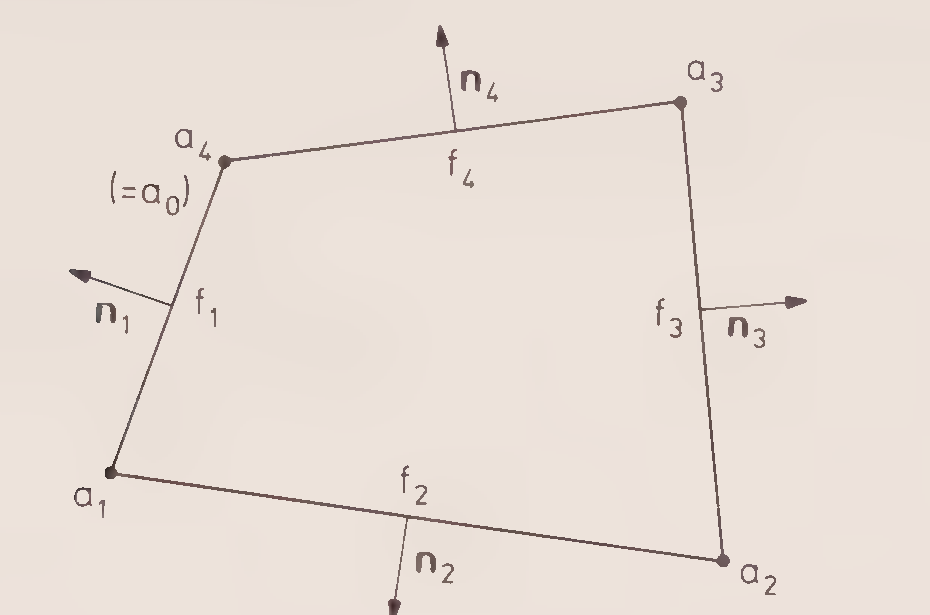
\includegraphics[width=.58\linewidth]{figures/chapter-02-figure-10.png}
\caption{四边形 $\kappa$ 的顶点、边和单位外法向量.}
\label{fig:primitive-quadrilateral-geometry}
\end{figure}

现在要寻找与 $\kappa$ 上常压力相容的速度向量 $\mathbf w$. 根据
Subsection~\ref{subsec:primitive-triangle-first-order} 的材料, $\mathbf w$
很可能属于比 $Q_1(\kappa)^2$ 更大的空间, 但它在 $\kappa$ 每条边上的切向分量应为仿射函数.
(事实上, 空间对 $(Q_1(\kappa)^2,P_0)$ 将是
Subsection~\ref{subsec:primitive-q1-p0-element} 的研究对象.) 例如, 参考正方形
$\hat\kappa$ 上的多项式
\[
\hat q_1=\hat\lambda_2\hat\lambda_3\hat\lambda_4
\]
在边 $\hat f_2,\hat f_3,\hat f_4$ 上为零. 因而函数
\[
\mathbf p_1=\mathbf n_1(\hat q_1\circ F_\kappa^{-1})
\]
在 $\kappa$ 的各边上具有零切向分量. 推广这一观察, 令
\begin{equation}\label{eq:primitive-quadrilateral-bubbles}
\begin{gathered}
\hat q_2=\hat\lambda_3\hat\lambda_4\hat\lambda_1,
\qquad
\hat q_3=\hat\lambda_4\hat\lambda_1\hat\lambda_2,
\qquad
\hat q_4=\hat\lambda_1\hat\lambda_2\hat\lambda_3,\\
\mathbf p_i=\mathbf n_i(\hat q_i\circ F_\kappa^{-1}),
\end{gathered}
\end{equation}
并在如下空间(维数为 12)中选取速度 $\mathbf w$:
\begin{equation}\label{eq:primitive-quadrilateral-first-local-space}
\mathcal Q_1(\kappa)=Q_1(\kappa)^2
\oplus\operatorname{span}\{\mathbf p_1,\mathbf p_2,\mathbf p_3,\mathbf p_4\}
\subset Q_2(\kappa)^2.
\end{equation}
如下一个 Lemma 所示, 与此空间自然联系的自由度为 $\mathbf w$ 在顶点 $a_i$
处的值以及 $\mathbf w$ 通过 $\kappa$ 每条边 $f_i$ 的通量.

\setcounter{statement}{0}
\renewcommand{\theHstatement}{lemma.\thesection.\arabic{statement}}
\begin{Lemma}\label{lem:primitive-quadrilateral-first-unisolvence}
$\mathcal Q_1(\kappa)$ 中的多项式 $\mathbf p$ 由以下 12 个量唯一确定:
\begin{equation}\label{eq:primitive-quadrilateral-first-dofs}
\left\{
\begin{aligned}
\mathbf p(a_i),&\qquad 1\leq i\leq4,\\
\int_{f_i}\mathbf p\cdot\mathbf n_i\,ds,&\qquad1\leq i\leq4.
\end{aligned}
\right.
\end{equation}
此外, $\mathbf p$ 在任一边 $f_i$ 上的限制只依赖于定义在该边上的自由度.
\end{Lemma}

\MathBookSourcePage{168}
\begin{Proof}
由于函数 $\mathbf p_i$ 在 $\kappa$ 的所有顶点上为零, 可写成
\begin{equation}\label{eq:primitive-quadrilateral-first-decomposition}
\mathbf p=I_\kappa\mathbf p+\sum_{i=1}^{4}\alpha_i\mathbf p_i,
\qquad \alpha_i\in\mathbb R,
\end{equation}
其中 $I_\kappa$ 表示 $Q_1(\kappa)^2$ 上的标准插值算子. 此外,
\begin{equation}\label{eq:primitive-quadrilateral-first-normal-trace}
(\mathbf p-I_\kappa\mathbf p)\cdot\mathbf n_i|_{f_i}
=\alpha_i(\hat q_i\circ F_\kappa^{-1})|_{f_i}.
\end{equation}
由这两个表达式立即可知, 所有自由度为零时只有零多项式.
\end{Proof}

于是选取如下速度和压力空间:
\begin{equation}\label{eq:primitive-quadrilateral-first-velocity-spaces}
\left\{
\begin{aligned}
W_h&=\{\,\mathbf w\in\mathcal C^0(\bar\Omega)^2;
\ \mathbf w|_\kappa\in\mathcal Q_1(\kappa)
\quad\forall\kappa\in\mathcal T_h\,\},\\
X_h&=W_h\cap H_0^1(\Omega)^2,
\end{aligned}
\right.
\end{equation}
\begin{equation}\label{eq:primitive-quadrilateral-first-pressure-spaces}
\left\{
\begin{aligned}
Q_h&=\{\,q\in L^2(\Omega);\ q|_\kappa\in P_0
\quad\forall\kappa\in\mathcal T_h\,\},\\
M_h&=Q_h\cap L_0^2(\Omega).
\end{aligned}
\right.
\end{equation}

Lemma~\ref{lem:primitive-quadrilateral-first-unisolvence} 提示在
$\mathcal Q_1(\kappa)$ 上定义插值算子 $r_\kappa$:
\[
r_\kappa\mathbf v(a_i)=\mathbf v(a_i),
\qquad
\int_{f_j}(r_\kappa\mathbf v-\mathbf v)\cdot\mathbf n_j\,ds=0,
\quad1\leq i<j\leq4.
\]
但这个算子仍不满足 Hypothesis H3, 因为它未定义在 $H^1(\Omega)^2$ 上.
因此, 与单纯形情形一样, 我们用类似于
Subsection~\ref{sec:appendix-interpolation-discontinuous-functions} 中算子的局部正则化算子
$R_h$ 的值替代上述 $\mathbf v$ 的值:
\[
R_h\in\mathcal L(H_0^1(\Omega);\Phi_h),
\]
其中
\[
\Phi_h=\{\,\phi\in\mathcal C^0(\bar\Omega);
\ \phi|_\kappa\in Q_1(\kappa)\quad\forall\kappa\in\mathcal T_h\,\}
\cap H_0^1(\Omega).
\]
再定义算子 $\pi_h\in\mathcal L(H_0^1(\Omega)^2;X_h)$:
\begin{equation}\label{eq:primitive-quadrilateral-first-fortin-operator}
\left\{
\begin{aligned}
\pi_h\mathbf v(a)&=R_h\mathbf v(a)
&&\text{对 $\mathcal T_h$ 的每个节点 $a$},\\
\int_f(\pi_h\mathbf v-\mathbf v)\cdot\mathbf n\,ds&=0
&&\text{对 $\mathcal T_h$ 的每条边 $f$}.
\end{aligned}
\right.
\end{equation}

为建立 $\pi_h$ 的逼近性质, 必须假设三角剖分 $\mathcal T_h$ 依照
Definition~\ref{def:appendix-regular-triangulation} 是正则的, 其参数为
\[
h_\kappa=\operatorname{diameter}(\kappa),
\qquad
\rho_\kappa=2\min_{1\leq i\leq4}
\{\operatorname{diameter}(S_i\text{ 的内切圆})\},
\]
其中 $S_i$ 表示顶点为 $a_{i-1},a_i,a_{i+1}$ 的三角形.

\setcounter{statement}{1}
\renewcommand{\theHstatement}{lemma.\thesection.\arabic{statement}}
\begin{Lemma}\label{lem:primitive-quadrilateral-first-fortin-estimates}
由 \eqref{eq:primitive-quadrilateral-first-fortin-operator} 定义的算子 $\pi_h$ 满足
\[
\int_\Omega\operatorname{div}(\mathbf v-\pi_h\mathbf v)q\,dx=0
\qquad\forall q\in Q_h.
\]

\MathBookSourcePage{169}
此外, 若三角剖分 $\mathcal T_h$ 正则, 则 $\pi_h$ 满足误差界
\begin{equation}\label{eq:primitive-quadrilateral-first-interpolation-error}
|\mathbf v-\pi_h\mathbf v|_{m,\Omega}
\leq Ch^{k-m}|\mathbf v|_{k,\Omega}
\qquad\forall\mathbf v\in H^k(\Omega)^2,
\end{equation}
其中 $m=0$ 或 $1$, 且 $k=1$ 或 $2$.
\end{Lemma}

\begin{Proof}
由 \eqref{eq:primitive-quadrilateral-first-decomposition} 和
\eqref{eq:primitive-quadrilateral-first-normal-trace} 得
\[
\pi_h\mathbf v=R_h\mathbf v+\sum_{i=1}^{4}\alpha_i\mathbf p_i,
\]
其中
\[
\alpha_i=
\left[\int_{f_i}(\mathbf v-R_h\mathbf v)\cdot\mathbf n_i\,ds\right]
\left/\int_{f_i}\hat q_i\circ F_\kappa^{-1}\,ds\right. .
\]
一方面, 对 $\mathbf v\in H^k(\Omega)^2$, 算子 $R_h$ 具有局部插值误差
\begin{equation}\label{eq:primitive-quadrilateral-regularization-error}
\|\mathbf v-R_h\mathbf v\|_{0,\kappa}
+h_\kappa|\mathbf v-R_h\mathbf v|_{1,\kappa}
\leq C_1h_\kappa^k|\mathbf v|_{k,\Delta_\kappa},
\qquad k=1\text{ 或 }2,
\end{equation}
其中 $\Delta_\kappa$ 仍表示至少与 $\kappa$ 共享一个顶点的四边形之并.

另一方面, Lemma~\ref{lem:appendix-quadrilateral-change-of-variables} 给出
\[
|\mathbf p_i|_{m,\kappa}
\leq C_2\sigma_\kappa^{2m}h_\kappa^{1-m}|\hat q_i|_{m,\hat\kappa}
\leq C_3\sigma_\kappa^{2m}h_\kappa^{1-m},
\qquad m=0\text{ 或 }1.
\]
此外,
\[
\int_{f_i}\hat q_i\circ F_\kappa^{-1}\,ds
=\operatorname{meas}(f_i)\int_{\hat f_i}\hat q_i\,d\hat s,
\]
并且
\[
\left|\int_{f_i}(\mathbf v-R_h\mathbf v)\cdot\mathbf n_i\,ds\right|
\leq\operatorname{meas}(f_i)
\int_{\hat f_i}\|\hat{\mathbf v}-\widehat{R_h\mathbf v}\|\,d\hat s,
\]
因为 $F_\kappa$ 在 $\kappa$ 的边上的限制是仿射的. 应用 trace
Theorem~\ref{thm:trace-operator} 和
Lemma~\ref{lem:appendix-quadrilateral-change-of-variables}, 得
\[
\int_{\hat f_i}\|\hat{\mathbf v}-\widehat{R_h\mathbf v}\|\,d\hat s
\leq(C_4/\rho_\kappa)
\{\|\mathbf v-R_h\mathbf v\|_{0,\kappa}^2
+h_\kappa^2|\mathbf v-R_h\mathbf v|_{1,\kappa}^2\}^{1/2}.
\]
因此 \eqref{eq:primitive-quadrilateral-regularization-error} 给出
\[
\left|\int_{f_i}(\mathbf v-R_h\mathbf v)\cdot\mathbf n_i\,ds\right|
\leq C_5\sigma_\kappa\operatorname{meas}(f_i)
h_\kappa^{k-1}|\mathbf v|_{k,\Delta_\kappa}.
\]
于是
\[
|\alpha_i|\leq C_6\sigma_\kappa h_\kappa^{k-1}|\mathbf v|_{k,\Delta_\kappa},
\qquad
|\alpha_i|\,|\mathbf p_i|_{m,\kappa}
\leq C_7\sigma_\kappa^{2m+1}h_\kappa^{k-m}|\mathbf v|_{k,\Delta_\kappa}.
\]
其余证明与 Lemma~\ref{lem:primitive-bernardi-raugel-fortin-estimates}
的证明相同.
\end{Proof}

\MathBookSourcePage{170}
最后, 上述空间 $Q_h$ 仍满足界 \eqref{eq:primitive-bernardi-raugel-pressure-projection}.
因此已经证明该格式为一阶格式.

\setcounter{statement}{0}
\renewcommand{\theHstatement}{theorem.\thesection.\arabic{statement}}
\begin{Theorem}\label{thm:primitive-quadrilateral-first-convergence}
设 $\Omega$ 是有界多边形, 并假设 Stokes 方程的解 $(\mathbf u,p)$ 满足
\[
\mathbf u\in[H^2(\Omega)\cap H_0^1(\Omega)]^2,
\qquad p\in H^1(\Omega)\cap L_0^2(\Omega).
\]
若三角剖分 $\mathcal T_h$ 正则, 则采用
\eqref{eq:primitive-quadrilateral-first-velocity-spaces} 和
\eqref{eq:primitive-quadrilateral-first-pressure-spaces} 所定义空间时,
\eqref{eq:primitive-discrete-q-first}--\eqref{eq:primitive-discrete-p}
的解 $(\mathbf u_h,p_h)$ 满足 Theorem~\ref{thm:primitive-bernardi-raugel-convergence}
的结论.
\end{Theorem}

\subsection{高阶四边形单元}
\label{subsec:primitive-quadrilateral-higher-order}

我们讨论并推广广泛使用的 ``$Q_2$--$P_1$'' 有限元格式. 简言之,
该方法采用连续速度, 其分量在每个单元 $\kappa$ 上为分片 $Q_2(\kappa)$,
同时采用在每个单元上分片属于 $P_1$ 的不连续压力. 它的分析相当直接,
而且容易推广到任意阶 $l$, 因此可直接从一般情形开始.

仍取 $\mathcal T_h$ 中任意四边形 $\kappa$, 并令
\begin{equation}\label{eq:primitive-quadrilateral-higher-velocity-spaces}
\left\{
\begin{aligned}
W_h&=\{\,\mathbf w\in\mathcal C^0(\bar\Omega)^2;
\ \mathbf w|_\kappa\in Q_l(\kappa)^2
\quad\forall\kappa\in\mathcal T_h\,\},\\
X_h&=W_h\cap H_0^1(\Omega)^2,
\end{aligned}
\right.
\end{equation}
\begin{equation}\label{eq:primitive-quadrilateral-higher-pressure-spaces}
\left\{
\begin{aligned}
Q_h&=\{\,q\in L^2(\Omega);
\ q|_\kappa\in P_{l-1}\quad\forall\kappa\in\mathcal T_h\,\},\\
M_h&=Q_h\cap L_0^2(\Omega),
\end{aligned}
\right.
\end{equation}
其中 $l\geq2$.

立即注意到 $\bar X_h\subset X_h$, 因而只需在局部检验 inf-sup 条件.
于是可以采用最简单的自由度, 例如: $\mathbf w$ 的每个分量在 $l$ 阶主格
$\Sigma_\kappa$ 上的值; 以及对 $q$ 与 $P_{l-1}$ 对应的矩
\[
\int_\kappa qf\,dx\qquad\forall f\in P_{l-1}.
\]
先建立局部 inf-sup 条件. 这里仍以三角剖分作为分割:
\begin{equation}\label{eq:primitive-quadrilateral-local-inf-sup-spaces}
\left\{
\begin{aligned}
X_h(\kappa)&=\{\,\mathbf v\in Q_l(\kappa)^2;
\ \mathbf v|_{\partial\kappa}=0\,\},\\
M_h(\kappa)&=P_{l-1}\cap L_0^2(\kappa).
\end{aligned}
\right.
\end{equation}

\setcounter{statement}{1}
\renewcommand{\theHstatement}{theorem.\thesection.\arabic{statement}}
\begin{Theorem}\label{thm:primitive-quadrilateral-local-inf-sup}
设三角剖分 $\mathcal T_h$ 正则. 则由
\eqref{eq:primitive-quadrilateral-local-inf-sup-spaces} 定义的空间对
$(X_h(\kappa),M_h(\kappa))$ 满足 Hypothesis H4.
\end{Theorem}

\MathBookSourcePage{171}
\begin{Proof}
证明与 Theorem~\ref{thm:primitive-triangle-local-inf-sup} 的证明大体相同,
这里只详述四边形所特有的细节. 有
\[
\begin{aligned}
\int_\kappa q\operatorname{div}\mathbf v\,dx
&=-\int_\kappa\mathbf v\cdot\operatorname{grad}q\,dx\\
&=-\int_{\hat\kappa}J_{F_\kappa}\hat{\mathbf v}\cdot
[(\operatorname{grad}q)\circ F_\kappa],d\hat x.
\end{aligned}
\]
由于 $q\in P_{l-1}$, 有 $\operatorname{grad}q\in P_{l-2}^2$, 从而
\[
(\operatorname{grad}q)\circ F_\kappa\in Q_{l-2}^2
\qquad\text{在 }\hat\kappa\text{ 上}.
\]
令
\[
b(\hat x)=\hat\lambda_1\hat\lambda_2\hat\lambda_3\hat\lambda_4
\]
表示 $\hat\kappa$ 上的``泡函数'', 并取
\[
\hat{\mathbf v}=-b(\hat x)[(\operatorname{grad}q)\circ F_\kappa].
\]
于是 $\mathbf v\in X_h(\kappa)$, 且
\[
\int_\kappa q\operatorname{div}\mathbf v\,dx
=\int_{\hat\kappa}J_{F_\kappa}b(\hat x)
\|(\operatorname{grad}q)\circ F_\kappa\|^2,d\hat x.
\]
映射
\[
\phi\longmapsto\int_{\hat\kappa}b(\hat x)|\phi|\,d\hat x
\]
在任意有限维空间上显然是范数, 因而
\[
\int_\kappa q\operatorname{div}\mathbf v\,dx
\geq C_1\int_{\hat\kappa}J_{F_\kappa}
\|(\operatorname{grad}q)\circ F_\kappa\|^2,d\hat x
\geq C_1|q|_{1,\kappa}^2.
\]
此外,
\[
\|\mathbf v\|_{0,\kappa}\leq|q|_{1,\kappa},
\qquad
|\mathbf v|_{1,\kappa}
\leq C_2(\sigma_\kappa^2/\rho_\kappa)\|\mathbf v\|_{0,\kappa},
\]
其中第二式由将 Lemma~\ref{lem:appendix-local-inverse-inequality}
的简单论证用于四边形得到. 因此
\[
\int_\kappa q\operatorname{div}\mathbf v\,dx
\geq C_3(\rho_\kappa/\sigma_\kappa^2)|q|_{1,\kappa}.
\]
所需结果于是由下一个 Lemma 和 $\mathcal T_h$ 的正则性得到.
\end{Proof}

\MathBookSourcePage{172}
\setcounter{statement}{2}
\renewcommand{\theHstatement}{lemma.\thesection.\arabic{statement}}
\begin{Lemma}\label{lem:primitive-quadrilateral-poincare}
设 $\kappa$ 是平面凸四边形. 存在与 $h$ 和 $\kappa$ 无关的常数 $C>0$, 使
\begin{equation}\label{eq:primitive-quadrilateral-poincare}
\|q\|_{0,\kappa}\leq C\sigma_\kappa h_\kappa|q|_{1,\kappa}
\qquad\forall q\in H^1(\kappa)\cap L_0^2(\kappa).
\end{equation}
\end{Lemma}

证明略去, 因为它与 Lemma~\ref{lem:primitive-simplex-scaled-poincare}
的证明完全相同.

还需考察 $W_h$ 和 $Q_h$ 的逼近性质. $W_h$ 中的逼近误差完全是标准的,
因为它直接来自 \eqref{eq:appendix-quadrilateral-lagrange-error-wsp}:
\begin{equation}\label{eq:primitive-quadrilateral-higher-velocity-interpolation}
|\mathbf w-I_h\mathbf w|_{m,\Omega}
\leq Ch^{k+1-m}|\mathbf w|_{k+1,\Omega}
\quad\forall\mathbf w\in H^{k+1}(\Omega)^2,
\quad1\leq k\leq l,
\quad m=0\text{ 或 }1.
\end{equation}
但 $Q_h$ 中的逼近误差并非如此直接, 因为这里在四边形(而不是三角形)上处理
$P_{l-1}$ 中的多项式. 特别地, Theorem~\ref{thm:appendix-quadrilateral-bramble-hilbert}
不能应用, 因为 $\{p\circ F_\kappa;p\in P_{l-1}\}$ 是 $Q_{l-1}$ 的真子空间.
下面的 Lemma 由 Bernardi 提供(私人通信).

\setcounter{statement}{3}
\renewcommand{\theHstatement}{lemma.\thesection.\arabic{statement}}
\begin{Lemma}\label{lem:primitive-quadrilateral-pressure-projection}
若三角剖分 $\mathcal T_h$ 正则, 则 $Q_h$ 上的 $L^2$ 正交投影算子 $\rho_h$ 满足
\begin{equation}\label{eq:primitive-quadrilateral-pressure-projection}
\|f-\rho_hf\|_{0,\Omega}
\leq Ch^k|f|_{k,\Omega}
\qquad\forall f\in H^k(\Omega),
\quad0\leq k\leq l.
\end{equation}
\end{Lemma}

\begin{Proof}
设 $\kappa$ 是 $\mathcal T_h$ 中的一个四边形. 注意, 若映射 $F_\kappa$
为仿射而不是双线性的, \eqref{eq:primitive-quadrilateral-pressure-projection}
便是平凡的. 因此我们将引入另一个映射.

\begin{figure}[htbp]
\centering
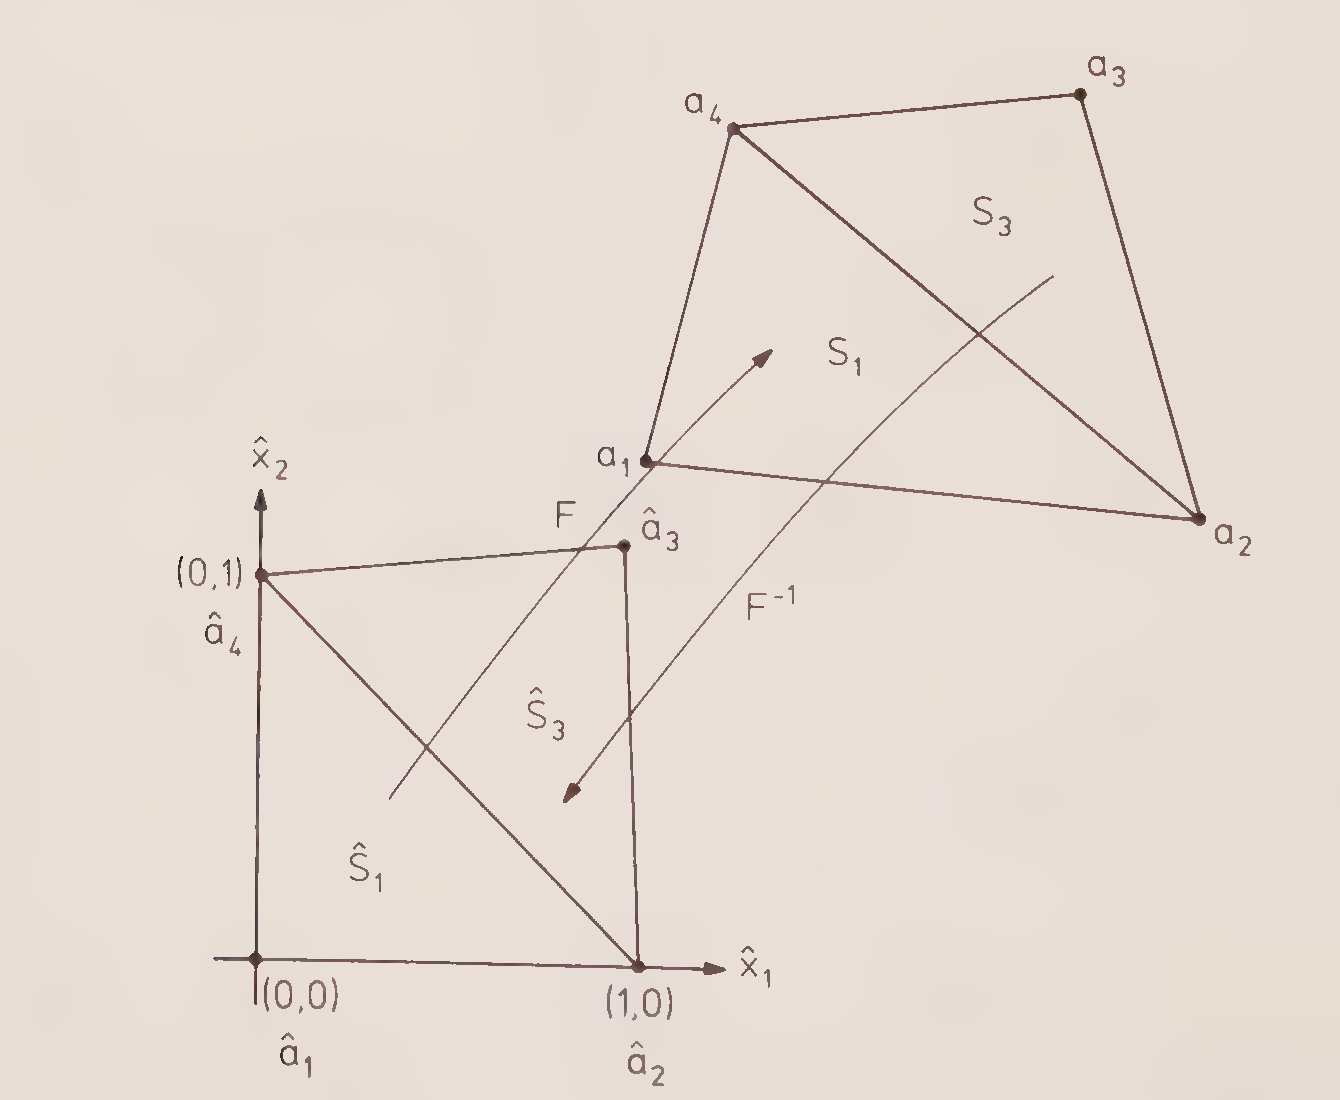
\includegraphics[width=.58\linewidth]{figures/chapter-02-figure-11.png}
\caption{四边形与参考正方形上的仿射子三角形.}
\label{fig:primitive-quadrilateral-affine-subtriangles}
\end{figure}
